% Options for packages loaded elsewhere
\PassOptionsToPackage{unicode}{hyperref}
\PassOptionsToPackage{hyphens}{url}
%
\documentclass[
  english,
  man,floatsintext]{apa6}
\usepackage{amsmath,amssymb}
\usepackage{lmodern}
\usepackage{ifxetex,ifluatex}
\ifnum 0\ifxetex 1\fi\ifluatex 1\fi=0 % if pdftex
  \usepackage[T1]{fontenc}
  \usepackage[utf8]{inputenc}
  \usepackage{textcomp} % provide euro and other symbols
\else % if luatex or xetex
  \usepackage{unicode-math}
  \defaultfontfeatures{Scale=MatchLowercase}
  \defaultfontfeatures[\rmfamily]{Ligatures=TeX,Scale=1}
\fi
% Use upquote if available, for straight quotes in verbatim environments
\IfFileExists{upquote.sty}{\usepackage{upquote}}{}
\IfFileExists{microtype.sty}{% use microtype if available
  \usepackage[]{microtype}
  \UseMicrotypeSet[protrusion]{basicmath} % disable protrusion for tt fonts
}{}
\makeatletter
\@ifundefined{KOMAClassName}{% if non-KOMA class
  \IfFileExists{parskip.sty}{%
    \usepackage{parskip}
  }{% else
    \setlength{\parindent}{0pt}
    \setlength{\parskip}{6pt plus 2pt minus 1pt}}
}{% if KOMA class
  \KOMAoptions{parskip=half}}
\makeatother
\usepackage{xcolor}
\IfFileExists{xurl.sty}{\usepackage{xurl}}{} % add URL line breaks if available
\IfFileExists{bookmark.sty}{\usepackage{bookmark}}{\usepackage{hyperref}}
\hypersetup{
  pdftitle={Great ape communication as contextual social inference: a computational modeling perspective},
  pdfauthor={Manuel Bohn1, Katja Liebal2, \& Michael Henry Tessler3,4},
  pdflang={en-EN},
  pdfkeywords={Communication, Primates, Social cognition, Evolution, Computational modeling},
  hidelinks,
  pdfcreator={LaTeX via pandoc}}
\urlstyle{same} % disable monospaced font for URLs
\usepackage{graphicx}
\makeatletter
\def\maxwidth{\ifdim\Gin@nat@width>\linewidth\linewidth\else\Gin@nat@width\fi}
\def\maxheight{\ifdim\Gin@nat@height>\textheight\textheight\else\Gin@nat@height\fi}
\makeatother
% Scale images if necessary, so that they will not overflow the page
% margins by default, and it is still possible to overwrite the defaults
% using explicit options in \includegraphics[width, height, ...]{}
\setkeys{Gin}{width=\maxwidth,height=\maxheight,keepaspectratio}
% Set default figure placement to htbp
\makeatletter
\def\fps@figure{htbp}
\makeatother
\setlength{\emergencystretch}{3em} % prevent overfull lines
\providecommand{\tightlist}{%
  \setlength{\itemsep}{0pt}\setlength{\parskip}{0pt}}
\setcounter{secnumdepth}{-\maxdimen} % remove section numbering
% Make \paragraph and \subparagraph free-standing
\ifx\paragraph\undefined\else
  \let\oldparagraph\paragraph
  \renewcommand{\paragraph}[1]{\oldparagraph{#1}\mbox{}}
\fi
\ifx\subparagraph\undefined\else
  \let\oldsubparagraph\subparagraph
  \renewcommand{\subparagraph}[1]{\oldsubparagraph{#1}\mbox{}}
\fi
% Manuscript styling
\usepackage{upgreek}
\captionsetup{font=singlespacing,justification=justified}

% Table formatting
\usepackage{longtable}
\usepackage{lscape}
% \usepackage[counterclockwise]{rotating}   % Landscape page setup for large tables
\usepackage{multirow}		% Table styling
\usepackage{tabularx}		% Control Column width
\usepackage[flushleft]{threeparttable}	% Allows for three part tables with a specified notes section
\usepackage{threeparttablex}            % Lets threeparttable work with longtable

% Create new environments so endfloat can handle them
% \newenvironment{ltable}
%   {\begin{landscape}\centering\begin{threeparttable}}
%   {\end{threeparttable}\end{landscape}}
\newenvironment{lltable}{\begin{landscape}\centering\begin{ThreePartTable}}{\end{ThreePartTable}\end{landscape}}

% Enables adjusting longtable caption width to table width
% Solution found at http://golatex.de/longtable-mit-caption-so-breit-wie-die-tabelle-t15767.html
\makeatletter
\newcommand\LastLTentrywidth{1em}
\newlength\longtablewidth
\setlength{\longtablewidth}{1in}
\newcommand{\getlongtablewidth}{\begingroup \ifcsname LT@\roman{LT@tables}\endcsname \global\longtablewidth=0pt \renewcommand{\LT@entry}[2]{\global\advance\longtablewidth by ##2\relax\gdef\LastLTentrywidth{##2}}\@nameuse{LT@\roman{LT@tables}} \fi \endgroup}

% \setlength{\parindent}{0.5in}
% \setlength{\parskip}{0pt plus 0pt minus 0pt}

% \usepackage{etoolbox}
\makeatletter
\patchcmd{\HyOrg@maketitle}
  {\section{\normalfont\normalsize\abstractname}}
  {\section*{\normalfont\normalsize\abstractname}}
  {}{\typeout{Failed to patch abstract.}}
\patchcmd{\HyOrg@maketitle}
  {\section{\protect\normalfont{\@title}}}
  {\section*{\protect\normalfont{\@title}}}
  {}{\typeout{Failed to patch title.}}
\makeatother
\shorttitle{A computational model of great ape communication}
\keywords{Communication, Primates, Social cognition, Evolution, Computational modeling}
\usepackage{lineno}

\linenumbers
\usepackage{csquotes}
\usepackage{setspace}
\captionsetup[figure]{font={stretch=1}}
\ifxetex
  % Load polyglossia as late as possible: uses bidi with RTL langages (e.g. Hebrew, Arabic)
  \usepackage{polyglossia}
  \setmainlanguage[]{english}
\else
  \usepackage[main=english]{babel}
% get rid of language-specific shorthands (see #6817):
\let\LanguageShortHands\languageshorthands
\def\languageshorthands#1{}
\fi
\ifluatex
  \usepackage{selnolig}  % disable illegal ligatures
\fi
\newlength{\cslhangindent}
\setlength{\cslhangindent}{1.5em}
\newlength{\csllabelwidth}
\setlength{\csllabelwidth}{3em}
\newenvironment{CSLReferences}[2] % #1 hanging-ident, #2 entry spacing
 {% don't indent paragraphs
  \setlength{\parindent}{0pt}
  % turn on hanging indent if param 1 is 1
  \ifodd #1 \everypar{\setlength{\hangindent}{\cslhangindent}}\ignorespaces\fi
  % set entry spacing
  \ifnum #2 > 0
  \setlength{\parskip}{#2\baselineskip}
  \fi
 }%
 {}
\usepackage{calc}
\newcommand{\CSLBlock}[1]{#1\hfill\break}
\newcommand{\CSLLeftMargin}[1]{\parbox[t]{\csllabelwidth}{#1}}
\newcommand{\CSLRightInline}[1]{\parbox[t]{\linewidth - \csllabelwidth}{#1}\break}
\newcommand{\CSLIndent}[1]{\hspace{\cslhangindent}#1}

\title{Great ape communication as contextual social inference: a computational modeling perspective}
\author{Manuel Bohn\textsuperscript{1}, Katja Liebal\textsuperscript{2}, \& Michael Henry Tessler\textsuperscript{3,4}}
\date{}


\affiliation{\vspace{0.5cm}\textsuperscript{1} Department of Comparative Cultural Psychology, Max Planck Institute for Evolutionary Anthropology\\\textsuperscript{2} Institute of Biology, Leipzig University\\\textsuperscript{3} Department of Brain and Cognitive Sciences, Massachusetts Institute of Technology\\\textsuperscript{4} DeepMind}

\abstract{
Human communication has been described as a contextual social inference process. Research into great ape communication has been inspired by this view to look for the evolutionary roots of the social, cognitive, and interactional processes involved in human communication. This approach has been highly productive, yet it is often compromised by a too-narrow focus on how great apes use and understand individual signals. In this paper, we introduce a computational model that formalizes great ape communication as a multi-faceted social inference process that relies on information contained in the signal, the relationship between communicative partners, and the social context. This model makes accurate qualitative and quantitative predictions about real-world communicative interactions between semi-wild-living chimpanzees. When enriched with a pragmatic reasoning process, the model explains repeatedly reported differences between humans and great apes in the interpretation of ambiguous signals (e.g.~pointing gestures). This approach has direct implications for observational and experimental studies of great ape communication and provides a new tool for theorizing about the evolution of uniquely human communication.
}



\begin{document}
\maketitle

\hypertarget{introduction}{%
\section{Introduction}\label{introduction}}

When discussing the origins of human communication, Levinson and colleagues {[}1,2{]} introduced the idea of a human \emph{interaction engine}. This metaphorical engine is assembled from a range of social-interactional parts that, when put together, enable uniquely human forms of communication, including conventional language. Each part was assumed to have deep roots in our evolutionary history and might therefore -- in one form or the other -- also be found in other primates. Inspired by these ideas, this paper introduces a computational model that specifies the role that social-interactional processes play in great ape and human communication.

What does the human interaction engine run on? First and foremost, human communication is seen as intentional. Senders produce signals to convey intentions and receivers use these signals to infer the sender's intentions {[}3--6{]}. As such, communication is deeply linked to reasoning about mental states. Signals, including conventional language, are used to express intentions but the link between signals and intentions is not rigid. There is always residual ambiguity that requires communicators to make additional (pragmatic) inferences -- a second key feature of human communication. Such inferences are licensed by a set of assumptions that humans hold about the nature of communication and social interaction more broadly. One such assumption is that communication occurs within some form of common ground -- a shared body of knowledge and beliefs that builds up during social interaction and serves as the background against which signals are interpreted {[}7,8{]}. Another assumption is that communication is cooperative such that senders choose their signals so that the receiver is more likely to infer the underlying intention. The receiver takes this into account when interpreting the signal.

The engine assembled from these -- and many other -- parts is independent of any particular modality. Multi-modality is seen as the norm, not an exception in human communication. The system is also highly flexible. Sometimes a tiny hand gesture might be enough to get a message across; at other times, the same meaning might require a long, elaborate utterance comprised of multiple signals that are combined according to conventional rules (grammar). Or as Levinson and Holler (2014) put it, ``The system remains highly flexible, allowing us to shift the burden from words to gestures as required by the current communicative needs.'' Many roads lead to Rome in human communication and \emph{what} works \emph{when} depends on the social-interactional embedding. The system is also independent of the availability of conventional (or evolved) signals. Conventional language is assumed to rely on the engine in just the same way as non-conventional communication. New signals can be invented and understood on the spot and later even conventionalized into new languages {[}9--15{]}.

The picture that emerges here provides an interesting starting point for an evolutionary research program because it decouples human communication from conventional language. The idea is that there is probably no direct link between the kind of signals our ancestors used (which might be comparable to what we see in great apes) and human language. The link lies in \emph{how} signals are used, that is, the social and cognitive underpinnings of communication. Once the interaction engine was in place, our ancestors started using and creating signals that, via intermediate proto-languages, evolved to become what we today see as conventional language {[}16--18{]}. Thus, instead of looking for structural features in animal communication that directly resemble aspects of conventional language (e.g.~arbitrary sound-to-meaning mappings or combinatorial syntax {[}19--23{]}, comparative researchers can ask which social-interactional processes underlie communication in other animals. In the next section, we will briefly summarize research in this tradition, with a focus on great ape communication.

\hypertarget{a-comparative-approach-to-human-language-the-intentional-nature-of-great-ape-communication}{%
\section{A comparative approach to human language: The intentional nature of great ape communication}\label{a-comparative-approach-to-human-language-the-intentional-nature-of-great-ape-communication}}

It is beyond the scope of this paper to give a comprehensive summary of existing research on primate communication. We will focus on two aspects that have been the focus of much comparative research: signalers' intentional signal production and recipients' extraction of the intended meaning of a signal. We will show that research on these two aspects of great ape communication varies drastically depending on whether the focus is on vocal, gestural, or facial signals. To make matters worse, there are also marked differences between research focusing on the production versus the perception or comprehension of signals.

To identify acts of intentional communication in great apes and other nonhuman primates, Leavens and colleagues {[}24{]} suggested a set of criteria derived from research on pre-linguistic communication in human infants {[}25{]}. These include the sender's sensitivity to the presence of other individuals, visual orienting behavior and monitoring of the recipient, the adjustment of signal use to the recipient's attentional state, and the use of attention-getting behaviors if recipients are not visually attending. Finally, senders are expected to continue signaling and to elaborate signal use in case initial communicative attempts fail.

There is now ample evidence that great apes are intentional communicators in that sense, not only in the gestural modality {[}26,27{]}. For example, several species of great apes adjust their signal use to the attentional state of the receiver and only deploy visual gestures if the recipient is attending {[}24,28{]}. They also wait for a response and persist in their communicative attempts and might even elaborate their gesture use if the receiver does not react {[}24,29,30{]}. Sumatran orang-utans use gestures and also some facial expressions flexibly to achieve a variety of social goals {[}31,32{]}. Furthermore, wild chimpanzees are more likely to produce alarm calls when other individuals are unaware of a potential threat {[}33,34{]}.

However, which and how many of the criteria for intentional communication are applied does not only vary across studies but also across modalities {[}26{]}. While intentional use is an integral part of defining a gesture, until more recently, this aspect was not considered important in vocal and facial research {[}35{]}, resulting in the common but unjustified dichotomy between intentional gestures and emotional vocalizations and facial expressions {[}6{]}.

The different theoretical and methodological approaches in vocal, gestural, and facial research have serious downstream consequences for research on primate communication more broadly. Gesture researchers focus on the behavior of the sender because of the importance of intentional signal production, while vocal and to a lesser extent also facial researchers focus on signal perception and how recipients extract a signal's meaning. Vocal researchers, for example, frequently use playback experiments to study recipients' reactions to a very specific call to identify the meaning or function of this call {[}36{]}. As a consequence, vocal researchers are interested in context-specific signals, with very specific meanings, while gesture researchers investigate the flexible use of one signal across different contexts and argue that the information conveyed by a gesture might differ depending on the context in which it is used. They further largely ignore context-specific signals, as this would not fulfill the criterion of flexible usage, which is often considered an additional marker of intentional use {[}26,31{]}.

Meaning is also conceptualized very differently across modalities, depending on whether the focus is on the signaler's or recipient's behavior {[}35{]}. While gesture researchers focus on the message the signaler intends to communicate, vocal (and partly also facial researchers) focus on the `meaning' extracted by the recipient {[}37,38{]}. As a consequence, it is difficult -- if not impossible -- to compare findings across modalities with regard to how nonhuman primates' communicative interactions are shaped by contextual information and how they `make sense' of others' communicative attempts.

Only more recently, there has been some cross-fertilization in both vocal and gesture research. Vocal researchers report that some vocalizations are less context-specific than previously thought {[}39{]}, while gesture researchers started to assign specific meanings to individual gestures {[}40,41{]}.

Despite these recent developments, it is important to highlight that research on primate communication has almost exclusively used a uni-modal approach: the majority of research focused either on gestural, vocal, or facial signals, and only very few studies investigated more than one signal modality simultaneously {[}42--45{]}.

There are a number of different reasons why researchers artificially break up the communicative process into components and study each of them in isolation {[}46{]}. For example, researchers are trained in both the theoretical approach and corresponding methods of their corresponding modality and there are also methodological constraints, as the methods used to study one modality (e.g., playback experiments) are not easily applicable to another modality.

There is, however, a deeper and more fundamental problem: we lack a theoretical account of how the different components integrate with one another. Therefore, many of the following questions remain unsolved. How do different signals relate to one another? How does the combination of a gesture with another signal (e.g.~gesture, facial expression, or vocalization) change the meaning or usage of the initial gesture? What role does the social context play? Our goal for the rest of the paper is to sketch out such a theoretical account in the form of a computational model. As a first step, we will briefly introduce the Rational Speech Act (RSA) framework which is used to study human linguistic communication and from which we took inspiration.

\hypertarget{computational-models-of-linguistic-communication-in-humans}{%
\section{Computational models of linguistic communication in humans}\label{computational-models-of-linguistic-communication-in-humans}}

A core challenge for a multi-layered, multi-modal system is to specify how the different information sources flow together. The RSA framework sees communication as a socially guided inference process {[}47,48{]}. A hypothetical listener in the model is assumed to reason about the intention that underlies the speaker's production of an utterance in context. Importantly, the listener assumes that the speaker is communicating in a cooperative way, choosing utterances that are maximally informative for the listener given the context. This assumption allows the listener to go beyond the literal meaning of the words that are used and to make pragmatic inferences.

The RSA framework has been successfully used to model a range of language understanding phenomena as pragmatic inferences including scalar and ad-hoc implicatures, non-literal language, politeness, and vagueness among others {[}47,49--53{]}. More recently, it has been used to predict how adults and children integrate different information sources to make inferences about what a speaker is referring to {[}54{]}. In one study, Bohn and colleagues {[}55{]} measured children's developing sensitivity to different information sources, for example, their linguistic knowledge or their sensitivity to common ground. They then used an RSA-type model to predict what should happen when people are confronted with multiple information sources at once. When they compared these predictions to new experimental data, they saw a very close alignment between the two, both qualitative and quantitative. To learn more about the integration process itself, they formalized a range of alternative models that varied in their assumptions about which information sources children used and how they integrate them. They found that children's behavior was best predicted by a model that assumed rational integration of all available information sources. Interestingly, the integration process was best described as stable across development. That is, even though children might change in how sensitive they are to different information sources, the way they integrate them seems to be stable across development. These studies illustrate how computational models can be used as a tool to study multi-layered communication.

For the model we describe below, we take inspiration from the RSA framework. The connection is mainly conceptual: we see communication as a socially guided inference process that relies on multiple, context-dependent information sources. There is, however, little structural overlap. In a later section, we explore how the social reasoning processes that are structural characteristics of RSA might be used to explain differences between great ape and human communication when it comes to interpreting novel and ambiguous signals.

\hypertarget{computational-models-of-primate-communication}{%
\section{Computational models of primate communication}\label{computational-models-of-primate-communication}}

Our main goal in this paper is to formulate a computational model of great ape communication. We focus on the in-the-moment comprehension of communicative acts. We ask how a receiver makes inferences about the intentions of a sender based on information contained in the signal, the relationship between communicative partners, and the social context. The process of in-the-moment comprehension has received little attention in previous modeling work in primate communication. We briefly review some of the earlier literature before laying out our approach.

Most formal work in primate communication has focused on modeling the production of different primate calls {[}56,57{]}. Though relevant for answering questions about the evolution of speech, this work does not help us understand the social-interactional nature of primate or ape communication. In a very ambitious project, Stuart Altmann\footnote{We are grateful to David Leavens for pointing us to Altmann's work.} {[}58{]} used stochastic models to predict the socio-communicative behavior of rhesus monkeys (\emph{Macaca mulatta}). He observed large groups of monkeys living on Cayo Santiago for two years with the goal to develop an ethogram of the species' social behavior. Next, he used his observations to define transitional probabilities between different behaviors. That is, he asked how well one can predict an individual's behavior if the previous behavior (by the same or another individual) is known. He did this for pairs of behaviors, but also for longer sequences. Perhaps unsurprisingly, he found that the behavioral stream is not a random sequence of events, but that behaviors cluster in a systematic way. In a very broad sense, we take this as an inspiration to look for a wider set of determinants when trying to predict in-the-moment comprehension and reactions.

Arbib and colleagues {[}59--62{]} focused specifically on gestural communication. Their main goal, however, was to model the ontogeny of gestures. Their model shows how behavioral patterns can evolve into communicative gestures during direct, physical interaction. Given their specific aim, the authors saw the gesture as the sole cause of changes in the receiver's behavior. Comprehension is treated as an associative learning process during which the observation of a particular action becomes paired with a particular reaction (i.e.~change in the receiver's goal state). The result is a linear mapping between observing a gesture and producing an outcome. In our model, we loosen this assumption and take into account that multiple information sources influence the response to a gesture.

\hypertarget{a-computational-model-of-chimpanzee-communication}{%
\section{A computational model of chimpanzee communication}\label{a-computational-model-of-chimpanzee-communication}}

In this section, we introduce a Bayesian computational model of great ape communication. In contrast to standard statistical procedures (e.g.~linear regression) which describe a particular data set, our model describes the inference processes we assume to underlie great apes' interpretation of communicative signals in context. These inference processes are built in to the model structure. Such a generative model can be used to predict and explain data sets (see below), but its main purpose is to provide a theoretical account of the phenomenon in question. In what follows, we first present a very general formulation of our model and then further specify it to capture a particular type of communicative interaction. We then evaluate the model based on an existing data set.

We see great ape communication as a contextualized social inference problem. That is, the sender produces an utterance which the receiver uses to make inferences about the sender's intention. Utterances can be composed of different types of signals coming from different modalities (e.g.~gestures, vocalizations, facial expressions, etc.). Inferences are contextualized in that, not just the utterance, but also the social context of the utterance as well as the relationship between the sender and receiver influence the receiver's interpretation. The model is formally defined as

\begin{equation}
P(i \mid u)\propto P(u \mid i) P(i)
\end{equation}

with \(P(i \mid u)\) being the probability that the sender has intention \(i\) given utterance \(u\). This decomposes into the likelihood of producing an utterance given an intention \(P(u \mid i)\) (e.g.~raising one's arm when wanting to be groomed) and the prior probability of having an intention in the first place \(P(i)\) (e.g.~wanting to be groomed). This very general formulation can be used as a framework to evaluate different hypotheses about which social information sources contribute to the likelihood and the prior; that is, which information sources play an important role in great ape communication.

Next, we spell out one variant of the model, which was influenced by the data set that we had available for evaluation. As mentioned above, the general framework could be used with more, fewer, or different information sources. For the purpose of the current paper, the likelihood is defined by the semantics associated with a gesture, \(\mathcal{L}(g,i)\), and a facial expression, \(\mathcal{L}(f,i)\), which independently contribute to make up the utterance:

\begin{equation}
P(u \mid i) = P(g,f \mid i) = \mathcal{L}(g,i \mid \theta_{g}) \mathcal{L}(f,i \mid \theta_{f})
\end{equation}

Signals have ``soft semantics'', that is, in contrast to a truth-functional (Boolean) semantics, we assume a probabilistic mapping between a signal and an intention (defined by the parameters \(\theta_{g}\) and \(\theta_{f}\)){[}63{]}. The utterance is contextualized by the prior probability of the intention, \(P(i)\), which we take to be a function of the context, and the social relation between individuals, \(P(i \mid c,s)\):

\begin{equation}
P(i)=P(i \mid c,s) = \rho_c \rho_s
\end{equation}

The direction and strength of the context and social relation components are defined by the parameters \(\rho_c\) and \(\rho_s\). In the example below, we provide more information about the interpretation of these parameters.

To evaluate the model, we used it to predict the outcome of communicative interactions between semi-wild-living chimpanzees (\emph{Pan troglodytes}). The data is taken from the study by Oña and colleagues {[}45{]} in which the authors observed two groups of chimpanzees (72 individuals) living in the Chimfunshi Wildlife Orphanage in Zambia. They focused on two types of manual gestures and investigated if combinations with a facial expression had a different meaning (measured as the context of usage and reaction of the recipient) compared to the single gesture. They recorded the communicative signals a sender produced, the context in which they were used and the reaction of the receiver. More specifically, they coded the type of manual gesture (stretched or bent arm), the facial expression (neutral, bared-teeth, or funneled-lip face), the social context of the interaction (positive or negative), and the dominance relationship between the sender and receiver (dominant or subordinate sender). They classified the outcome of the interaction as either affiliative or avoidant. For more details about the coding, we refer to the original publication.

As noted above, in our model, the gesture and the facial expressions contribute to the utterance (the likelihood) and the social context and the relationship contribute to the prior. We assigned parameter values to each of the components of the communicative interactions. The goal was to show that by choosing intuitive parameter values, our model can give rise to the data we observed. These values range between 0 and 1 and represent the degree with which a component is indicative of a positive (affiliative; 0 - 0.5) or negative (avoidant; 0.5 - 1) interpretation. We assumed the stretched-arm gesture to be weakly negative (\(\theta_{gs}\)= 0.53) and the bent-arm gesture to be weakly positive (\(\theta_{gb}\)= 0.47). Neutral facial expressions were set to be neutral (\(\theta_{fn}\)= 0.5), bared-teeth expressions were set to be weekly negative (\(\theta_{fb}\) = 0.6), and funneled-lip expressions to be strongly negative (\(\theta_{ff}\) = 0.9). A negative context was set to be negative (\(\rho_{cn}\) = 0.7) and a positive to be positive (\(\rho_{cp}\) = 0.3). Finally, we assumed that a positive reaction was likely for a dominant sender (\(\rho_{sd}\) = 0.25) and a negative outcome likely for a subordinate sender (\(\rho_{ss}\) = 0.75).

We want to highlight that even though these parameter values are inspired by prior work and common sense, they are to some extent arbitrary and should not be taken to reflect a strong commitment to the role the individual components might play in a different context. Their main purpose is to capture the idea that different components of the communicative interaction are more or less associated with a particular response. Code to run the model is available in the associated online repository: \url{https://github.com/manuelbohn/RSApes}.

Based on the model and the parameter settings we generated predictions for all possible combinations of gestures, facial expression, dominance relationship, and social context. We compared these predictions to the observations made by Oña and colleagues {[}45{]}. Our model makes predictions about the receiver's interpretation of the utterance in context. The data, however, only recorded the receivers' reactions. We assume that the receiver's reaction is guided by their interpretation of the utterance: When inferring a negative intention, the receiver shows an avoidant reaction and when inferring a positive intention, they show an affiliative reaction. Thus, for the purpose of the model comparison, we assume a one-to-one mapping between the interpretation of the sender's message and the receiver's reaction.

Observations in the data were not equally distributed across all possible combinations. To evaluate the model predictions, we focused on combinations that had at least five observations. All combinations that fulfilled this criterion were observed in a negative social context. When we compare the model predictions to the data, we therefore only visualize the negative context (Figure \ref{fig:fig1}). Note, however, that our model also generated predictions for the positive context.



\begin{figure}

{\centering 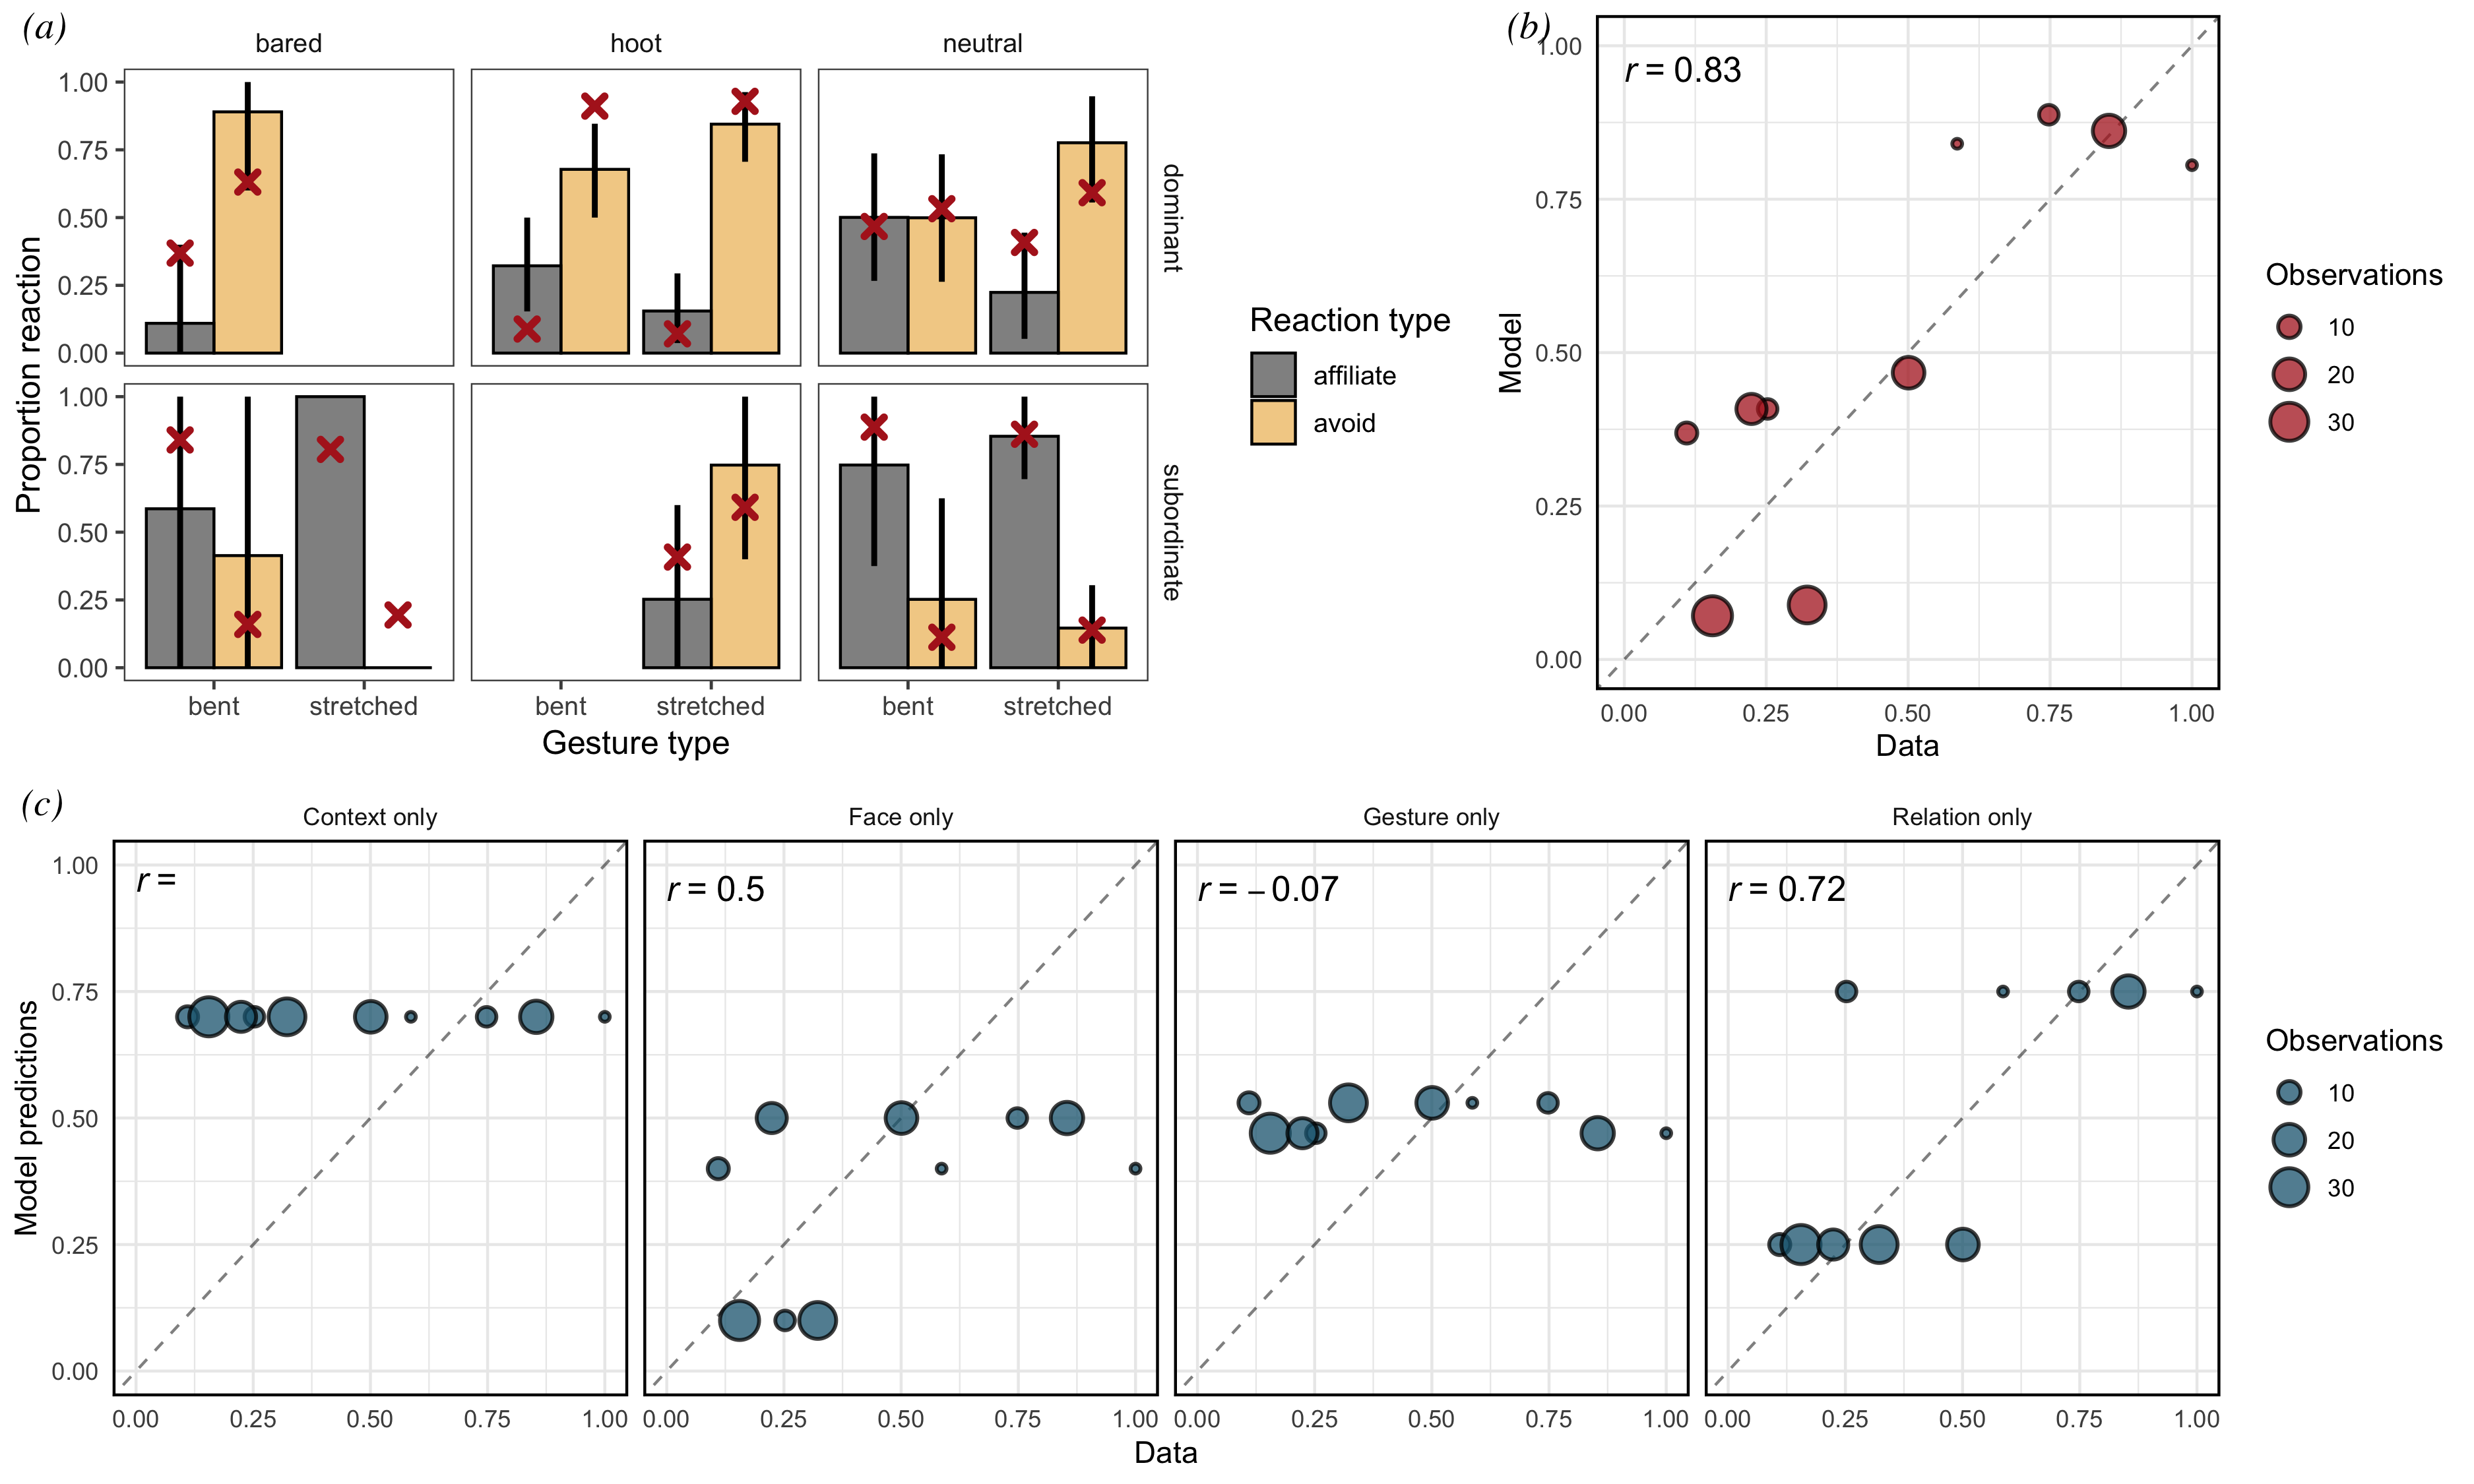
\includegraphics[width=1\linewidth]{../graphs/Fig1} 

}

\caption{Model predictions compared to data from {[}45{]}. Panel (a) shows the mean proportion (bars) of affiliative and avoidant reactions for combinations of gesture, facial expression, relationship, and social context in the data. Only combinations with more than 5 observations are shown. Error bars are 95\% Confidence Intervals based on a non-parametric bootstrap. Red crosses show model predictions. Panel (b) shows correlations between model prediction and data for avoidant reactions. The size of each point is proportional to the number of observations for a particular combination in the data. Panel (c) shows correlations for reduced models that focus only on a single component.}\label{fig:fig1}
\end{figure}

In Figure \ref{fig:fig1}, we can see that the model explains the data well, both quantitatively and qualitatively. The model predictions go in the same qualitative direction as the data, predicting more negative reactions when more negative reactions were observed. Furthermore, many of the model predictions also align quantitatively with the data, resulting in a high correlation between the two (Figure \ref{fig:fig1}b). Let us take a closer look at some of these patterns. In most cases, the qualitative pattern in the data was the same for both gesture types. For example, in a negative context, with a subordinate sender and a neutral facial expression, no matter if a bent or a stretched-arm gesture was used, there were more affiliative reactions. Our model predicts this pattern despite the fact that we took the stretched-arm gesture to be associated with a negative intention. The reason for this is that both gestures were assumed to have weak meanings. As a consequence, they had very little predictive power when a different, stronger information source (the dominance relationship in this case) was also available.

Next, we used this modeling framework to illustrate the theoretical point made above, namely that a focus on a single aspect of great ape communication is likely to yield an incomplete picture of the interaction. We formulated four reduced models, which use the same parameter settings as above, but selectively focused only on one of the components (all other parameters set to 0.5). When comparing the predictions from these reduced models to the data, we saw that none of them captured the data equally well compared to the full model\footnote{In the online repository, we also include a model in which the strength of the meaning of gestures and facial expressions was switched. That is, gestures were assumed to have a rather strong meaning and facial expressions a weak one. This model makes worse qualitative and quantitative predictions compared to one presented in the paper.} (Figure \ref{fig:fig1}c). Taken together, the results illustrate how computational modeling can be used as a powerful tool to study great ape communication. In the next section, we explore ways in which we can use this tool to theorize about some potential differences between ape and human communication.

\hypertarget{pragmatics-as-an-amplifier-in-human-communication}{%
\section{Pragmatics as an amplifier in human communication}\label{pragmatics-as-an-amplifier-in-human-communication}}

In their description of the interaction engine, Levinson and Holler {[}2{]} point out that ``language is the tip of an iceberg riding on a deep infrastructure of communicational abilities''. Part of this deep infrastructure is pragmatics. As noted in the introduction, the central idea is that utterances are not interpreted at face value, but that listeners go beyond the literal and make inferences about why the speaker produced a particular utterance in context. A cornerstone of this reasoning is the assumption that the speaker is cooperative and informative; they produce utterances that help the listener to infer their intention.

In the following, we enrich our model of great ape communication by pragmatics. From an evolutionary perspective, we may say that our great ape model stands in for the last common ancestor of great apes and humans. To recapitulate, we assume that this ancestor (and modern great apes) rationally integrated different information sources to make inferences about the sender's intentions. This includes information contained in the utterance as well as the social context and the relationship between communicators. The pragmatic abilities are built on top of this basic infrastructure to provide modern human communication.

To evaluate this pragmatically enriched model, we want to use it to explain some peculiar differences that have been reported for the communicative abilities of great apes and humans. Numerous studies have shown that great apes struggle to spontaneously understand ambiguous gestures, for example, pointing or novel iconic gestures {[}9,64--71{]} (with some particular exceptions {[}72,73{]}). These findings are peculiar because these gestures are naturally meaningful in that they either index (pointing) or resemble (iconic gestures) the referent. What is more, human children understand them spontaneously already very early in life {[}74,75{]}. Apes also seem to be somewhat sensitive to the natural meaning of these gestures. In the case of pointing, they often look in the direction the experimenter is pointing {[}76{]}. And in one study, iconic gestures were learned faster compared to arbitrary ones {[}77{]}.

Why do apes struggle with spontaneous comprehension of these gestures? The results of the model above can be taken to suggest that the social context and the relationship between sender and receiver play an important role in great ape communication. In the experimental setups of studies on pointing or iconic gesture comprehension, these components are controlled for and therefore offer no information about the sender's intention. Great apes are left with only the gesture. If that gesture was initially only vaguely associated with one or the other outcome, it would not provide sufficient information for apes to infer the sender's intention and thus to systematically select the referred-to object.

Why do humans spontaneously understand these gestures? We think that the notion of pragmatics as spelled out above can act as an amplifier of vague literal meanings. That is, a human receiver assumes that the speaker produced a particular gesture in a cooperative and informative manner to inform them about their intention. This line of argument is of course reminiscent of the idea that humans -- but not great apes -- are sensitive to cooperative communicative intentions {[}6{]}. However, we assume that pragmatic inferences just one information source that can be exploited and that they are graded -- not all or nothing. Next, we substantiate these ideas via our modeling framework.

The RSA framework introduced above is built around the assumptions that a) listeners reason about why speakers produce certain utterances and b) listeners assume that speakers communicate in a cooperative and informative way. This social reasoning component is formalized by embedding the model of the literal listener, \(P_{L_0}\), in a model of the speaker,\(P_{S_1}\). This \emph{pragmatic} speaker chooses utterances so that they are informative for the literal listener, while the literal listener simply interprets utterances in line with their literal semantics. This literal listener behaves exactly like in the great ape model. This illustrates the way in which our model of human communication is built around our model of great ape communication. At the highest level, we now have a pragmatic listener, \(P_{L_1}\). These additions change our model like so:

\begin{equation}
P_{L_1}(i \mid u)\propto P_{S_1}(u \mid i) P(i)
\label{eq:rsabasic1}
\end{equation}

\begin{equation}
P_{S_1}(u \mid i)\propto P_{L_0}(i\mid u) ^{\alpha_i}
\label{eq:rsabasic2}
\end{equation}

\begin{equation}
P_{L_0}(i\mid u) \propto \mathcal{L}(u, i \mid \theta_{u})
\label{eq:rsabasic3}
\end{equation}

Equation \eqref{eq:rsabasic2} above shows that the degree of how informative the speaker is assumed to be depends on the parameter \(\alpha\). The higher \(\alpha\), the more informative the speaker is assumed to be. The effect of \(\alpha\), however, depends on the presence of the speaker model, which represents the additional social reasoning component that we think is characteristic of human communication.



\begin{figure}

{\centering 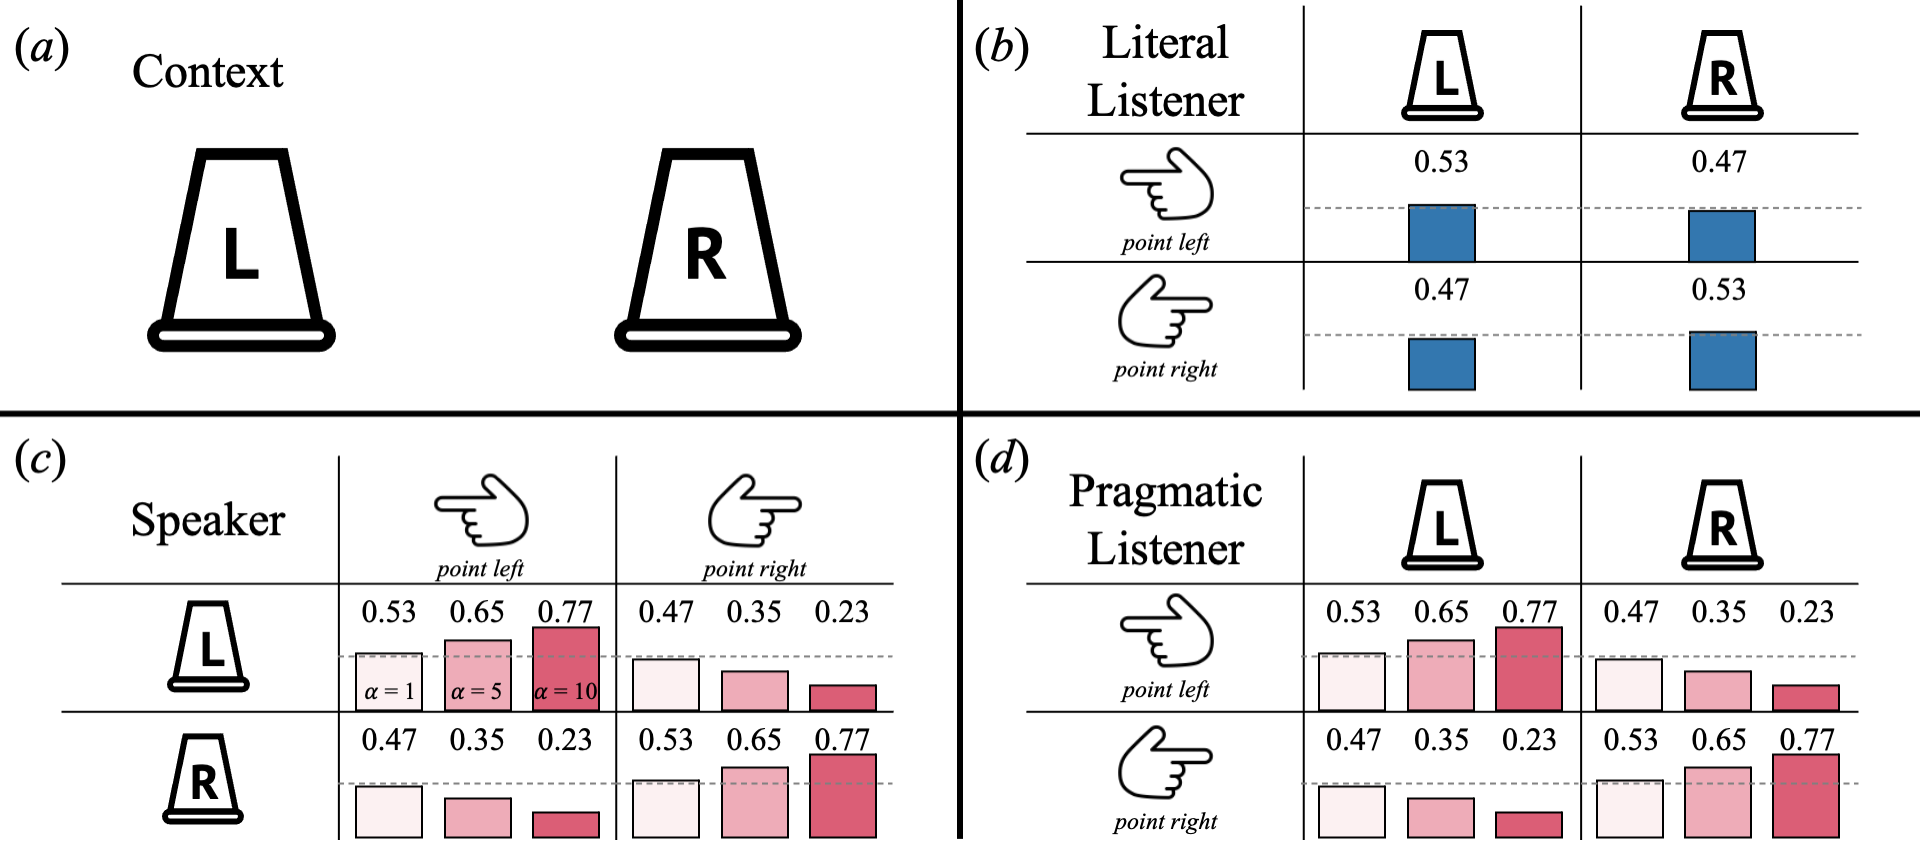
\includegraphics[width=1\linewidth]{../graphs/Fig2} 

}

\caption{Application of the pragmatically enriched model to an object-choice task with pointing gestures. Panel (a) shows the context with the two locations (L = left and R = right) that can be referred to. Panel (b) gives the interpretation probabilities of a literal listener. Panel (c) shows the production probabilities for the pragmatic speaker for values of \(\alpha\) = 1, 5, and 10. Panel (d) shows the interpretation probabilities of the pragmatic speaker based on the production probabilities in panel (c). Colored bars visualize the probabilities in reference to chance (grey dashed line). Different shades of red in (c) and (d) correspond to the magnitude of \(\alpha\).}\label{fig:fig2}
\end{figure}

When we adopt such a model to a situation in which the receiver is faced with a vaguely meaningful gesture (e.g.~a point or an iconic gesture; \(\theta_{u}\) = 0.53) without any additional contextual information, we see that the literal interpretation of the gesture simply reflects this vague meaning (Figure \ref{fig:fig2}b). We also see that pragmatic reasoning amplifies the initially vague meaning (Figure \ref{fig:fig2}d). As noted above, this is not due to the additional social reasoning component alone but critically depends on the receiver's expectation about cooperative communication (the parameter \(\alpha\), Figure \ref{fig:fig2}c). This highlights the graded relation between assumptions about cooperativeness and pragmatic inference. Once again, we would like to point out that the specific parameter values we picked here are arbitrary and do not reflect a strong commitment to how great apes or humans interpret pointing gestures. They simply serve to illustrate the point that pragmatics may amplify vague natural meanings.

\hypertarget{implications-and-future-directions}{%
\section{Implications and future directions}\label{implications-and-future-directions}}

Our goal in the modeling exercise presented above was twofold. On the one hand, we wanted to show that great ape communication is best thought of (and studied) as a multi-faceted, multi-modal, social inference process. We saw that the outcome of a communicative interaction was best predicted when signals, as well as contextual components, were taken into account. We do not say that studying these components in isolation is fruitless, but we do emphasize that focusing exclusively on, for example, the gesture or vocalization produced makes it less likely to understand the interaction that is unfolding. From our perspective, the different components play complementary roles in an integrated inference process.

Our hope is that our model proves to be a useful tool -- or at least an inspiration -- for future research. The approach by Oña and colleagues {[}45{]}, in which many different aspects of a communicative interaction are coded, seems to be especially promising. Such work could easily be done using already existing video recordings. Models like the one presented here could then be used to specify how the different components work together. In addition, our framework provides a new way to test competing hypotheses. Instead of relying on qualitative predictions, alternative hypotheses can be formalized as alternative models and then directly compared in a quantitative way. Across studies, it would be interesting to see if general patterns emerge. For example, models that emphasize social-contextual components could make better predictions compared to models emphasizing information provided by the utterance. Or models prioritizing facial expressions could be found to outcompete models that more strongly emphasize gestures. Or vice versa in both cases. Experimental studies could gradually vary the information provided by signals and the social context to study how they trade-off with one another. Such an approach might reveal gradual differences between humans and other primates where we currently assume qualitative ones In all of this, we think that the study of great ape communication would benefit from an interdisciplinary approach in which computational modelers work together with primatologists and comparative psychologists. Hopefully, this will allow the field to move away from asking somewhat artificial questions about the importance of individual gestures, facial expressions or vocalizations and instead move towards more comprehensive theories of the actual processes that underlie communicative interactions.

On the other hand, we have demonstrated how pragmatic reasoning can act as a gradual amplifier for signals with vague meanings. This perspective might be helpful for theorizing about the gradual transition from animal to human communication. For example, Sterelny {[}78{]} has argued that the transition from animal to human communication involved shifting from code-based to ostensive inferential communication {[}79{]}. During this process, the tight signal-response coupling characteristic for code-based communication was loosened. This brought an increase in flexibility, allowing senders to use the same signal for different and potentially novel purposes. However, it also introduced ambiguity to the signal, which, according to Sterelny, was compensated by relying on social reasoning processes. This transition shifted the locus of selection from specific signal-response couplings to communicative behavior more broadly. Our model formalizes the trade-off between ambiguity in the signal -- which is characteristic of human communication {[}18,80{]}-- and social reasoning. As such, it could be used as a starting point to formalize the gradual evolution of human ostensive-inferential communication.

The gradual emergence of pragmatic social reasoning in the evolution of human communication might have had further downstream consequences for the emergence of conventional communication systems. Recently, Hawkins and colleagues {[}81{]} embedded an RSA model of pragmatic in-the-moment inferences in a model of convention formation and showed how signals with vague meanings can give rise to conventional communication systems. The meaning of a signal can get fixed (e.g., further amplified) when it is repeatedly used within dyadic communicative interactions. Conventions form when partner-specific communicative conventions are gradually transferred, via a hierarchical Bayesian model, to novel communicative partners. Work by Woensdregt and colleagues {[}82{]} suggests that the presence of conventional communication systems further facilitates in-the-moment inferences about communicative intentions, leading to a cascading co-evolution of conventional language and social reasoning.

Finally, our modeling approach informs discussions about the modality in which human language has evolved. For decades, there has been a strong divide between researchers arguing for a vocal or a gestural origin of language {[}17,42,83{]}. Recently, the idea that language origins were multi-modal has gained traction. Our model provides a way of thinking about multi-modal communication. The model does not make any principled distinction between different modalities: for every signal, it simply asks how indicative it is for different intentions the sender might have. This explains how different signals influence each other during in-the-moment comprehension and could also be used to investigate how the burden may have shifted between modalities during the course of evolution.

\hypertarget{conclusion}{%
\section{Conclusion}\label{conclusion}}

Inspired by work on the human interaction engine, we have described a computational approach for how to study great ape communication in context. Our model assumes that great apes rationally integrate different information sources to make inferences about the intention behind a sender's utterance in context. Using existing data, we have shown that our model made accurate predictions about the outcome of multi-modal communicative interactions between chimpanzees in different social contexts. Based on the idea that pragmatic reasoning -- social reasoning paired with assumptions about cooperative communication -- acts as an amplifier for vague meanings, we suggested an explanation for some peculiar differences between the way that great apes and humans interpret ambiguous signals. This approach illustrates some deep similarities between human and great apes communication, but also specifies in what way the human interaction engine might be equipped with some special parts.

\newpage

\hypertarget{references}{%
\section{References}\label{references}}

\begingroup
\setlength{\parindent}{-0.5in}
\setlength{\leftskip}{0.5in}

\hypertarget{refs}{}
\begin{CSLReferences}{0}{0}
\leavevmode\hypertarget{ref-levinson2006human}{}%
\CSLLeftMargin{1. }
\CSLRightInline{Levinson SC. 2006 On the human {``interactional engine''}. In \emph{Roots of human sociality: culture, cognition and interaction} (eds N Enfield, S Levinson), pp. 39--69. Oxford : Berg. }

\leavevmode\hypertarget{ref-levinson2014origin}{}%
\CSLLeftMargin{2. }
\CSLRightInline{Levinson SC, Holler J. 2014 The origin of human multi-modal communication. \emph{Philosophical Transactions of the Royal Society B: Biological Sciences} \textbf{369}, 20130302.}

\leavevmode\hypertarget{ref-grice1991studies}{}%
\CSLLeftMargin{3. }
\CSLRightInline{Grice HP. 1991 \emph{Studies in the way of words}. Cambridge, MA: Harvard University Press. }

\leavevmode\hypertarget{ref-levinson2000presumptive}{}%
\CSLLeftMargin{4. }
\CSLRightInline{Levinson SC. 2000 \emph{Presumptive meanings: The theory of generalized conversational implicature}. Cambridge, MA: MIT press. }

\leavevmode\hypertarget{ref-sperber2001relevance}{}%
\CSLLeftMargin{5. }
\CSLRightInline{Sperber D, Wilson D. 2001 \emph{Relevance: Communication and cognition}. 2nd edn. Cambridge, MA: Blackwell Publishers. }

\leavevmode\hypertarget{ref-tomasello2008origins}{}%
\CSLLeftMargin{6. }
\CSLRightInline{Tomasello M. 2008 \emph{Origins of human communication}. Cambridge, MA: MIT press. }

\leavevmode\hypertarget{ref-bohn2018common}{}%
\CSLLeftMargin{7. }
\CSLRightInline{Bohn M, Köymen B. 2018 Common ground and development. \emph{Child Development Perspectives} \textbf{12}, 104--108.}

\leavevmode\hypertarget{ref-clark1996using}{}%
\CSLLeftMargin{8. }
\CSLRightInline{Clark HH. 1996 \emph{Using language}. Cambridge: Cambridge University Press. }

\leavevmode\hypertarget{ref-bohn2019natural}{}%
\CSLLeftMargin{9. }
\CSLRightInline{Bohn M, Call J, Tomasello M. 2019 Natural reference: A phylo-and ontogenetic perspective on the comprehension of iconic gestures and vocalizations. \emph{Developmental Science} \textbf{22}, e12757.}

\leavevmode\hypertarget{ref-bohn2019young}{}%
\CSLLeftMargin{10. }
\CSLRightInline{Bohn M, Kachel G, Tomasello M. 2019 Young children spontaneously recreate core properties of language in a new modality. \emph{Proceedings of the National Academy of Sciences} \textbf{116}, 26072--26077.}

\leavevmode\hypertarget{ref-brentari2017language}{}%
\CSLLeftMargin{11. }
\CSLRightInline{Brentari D, Goldin-Meadow S. 2017 Language emergence. \emph{Annual Review of Linguistics} \textbf{3}, 363--388.}

\leavevmode\hypertarget{ref-fay2014creating}{}%
\CSLLeftMargin{12. }
\CSLRightInline{Fay N, Lister CJ, Ellison TM, Goldin-Meadow S. 2014 Creating a communication system from scratch: Gesture beats vocalization hands down. \emph{Frontiers in Psychology} \textbf{5}, 354.}

\leavevmode\hypertarget{ref-goldin1977development}{}%
\CSLLeftMargin{13. }
\CSLRightInline{Goldin-Meadow S, Feldman H. 1977 The development of language-like communication without a language model. \emph{Science} \textbf{197}, 401--403.}

\leavevmode\hypertarget{ref-sandler2005emergence}{}%
\CSLLeftMargin{14. }
\CSLRightInline{Sandler W, Meir I, Padden C, Aronoff M. 2005 The emergence of grammar: Systematic structure in a new language. \emph{Proceedings of the National Academy of Sciences} \textbf{102}, 2661--2665.}

\leavevmode\hypertarget{ref-senghas2004children}{}%
\CSLLeftMargin{15. }
\CSLRightInline{Senghas A, Kita S, Özyürek A. 2004 Children creating core properties of language: Evidence from an emerging sign language in nicaragua. \emph{Science} \textbf{305}, 1779--1782.}

\leavevmode\hypertarget{ref-bar2013origins}{}%
\CSLLeftMargin{16. }
\CSLRightInline{Bar-on D. 2013 Origins of meaning: Must we {``go gricean''}? \emph{Mind \& Language} \textbf{28}, 342--375.}

\leavevmode\hypertarget{ref-fitch2010evolution}{}%
\CSLLeftMargin{17. }
\CSLRightInline{Fitch WT. 2010 \emph{The evolution of language}. Cambridge University Press. }

\leavevmode\hypertarget{ref-pleyer2017protolanguage}{}%
\CSLLeftMargin{18. }
\CSLRightInline{Pleyer M. 2017 Protolanguage and mechanisms of meaning construal in interaction. \emph{Language Sciences} \textbf{63}, 69--90.}

\leavevmode\hypertarget{ref-arbib2008primate}{}%
\CSLLeftMargin{19. }
\CSLRightInline{Arbib MA, Liebal K, Pika S. 2008 Primate vocalization, gesture, and the evolution of human language. \emph{Current Anthropology} \textbf{49}, 1053--1076.}

\leavevmode\hypertarget{ref-arnold2006semantic}{}%
\CSLLeftMargin{20. }
\CSLRightInline{Arnold K, Zuberbühler K. 2006 Semantic combinations in primate calls. \emph{Nature} \textbf{441}, 303--303.}

\leavevmode\hypertarget{ref-boe2017origins}{}%
\CSLLeftMargin{21. }
\CSLRightInline{Boë L-J, Fagot J, Perrier P, Schwartz J-L. 2017 \emph{Origins of human language: Continuities and discontinuities with nonhuman primates}. Peter Lang International Academic Publishers. }

\leavevmode\hypertarget{ref-fedurek2011primate}{}%
\CSLLeftMargin{22. }
\CSLRightInline{Fedurek P, Slocombe KE. 2011 Primate vocal communication: A useful tool for understanding human speech and language evolution? \emph{Human Biology} \textbf{83}, 153--173.}

\leavevmode\hypertarget{ref-zuberbuhler2005phylogenetic}{}%
\CSLLeftMargin{23. }
\CSLRightInline{Zuberbühler K. 2005 The phylogenetic roots of language: Evidence from primate communication and cognition. \emph{Current Directions in Psychological Science} \textbf{14}, 126--130.}

\leavevmode\hypertarget{ref-leavens2005intentionality}{}%
\CSLLeftMargin{24. }
\CSLRightInline{Leavens DA, Russell JL, Hopkins WD. 2005 Intentionality as measured in the persistence and elaboration of communication by chimpanzees (pan troglodytes). \emph{Child Development} \textbf{76}, 291--306.}

\leavevmode\hypertarget{ref-bates1979emergence}{}%
\CSLLeftMargin{25. }
\CSLRightInline{Bates E, Benigni L, Bretherton I, Camaioni L, Volterra V. 1979 \emph{The emergence of symbols: Cognition and communication in infancy}. New York: Academic Press. }

\leavevmode\hypertarget{ref-liebal2014primate}{}%
\CSLLeftMargin{26. }
\CSLRightInline{Liebal K, Waller BM, Burrows AM, Slocombe KE. 2014 \emph{Primate communication: A multimodal approach}. Cambridge University Press. }

\leavevmode\hypertarget{ref-townsend2017exorcising}{}%
\CSLLeftMargin{27. }
\CSLRightInline{Townsend SW \emph{et al.} 2017 Exorcising grice's ghost: An empirical approach to studying intentional communication in animals. \emph{Biological Reviews} \textbf{92}, 1427--1433.}

\leavevmode\hypertarget{ref-poss2006differential}{}%
\CSLLeftMargin{28. }
\CSLRightInline{Poss SR, Kuhar C, Stoinski TS, Hopkins WD. 2006 Differential use of attentional and visual communicative signaling by orangutans (pongo pygmaeus) and gorillas (gorilla gorilla) in response to the attentional status of a human. \emph{American Journal of Primatology} \textbf{68}, 978--992.}

\leavevmode\hypertarget{ref-cartmill2007orangutans}{}%
\CSLLeftMargin{29. }
\CSLRightInline{Cartmill EA, Byrne RW. 2007 Orangutans modify their gestural signaling according to their audience's comprehension. \emph{Current Biology} \textbf{17}, 1345--1348.}

\leavevmode\hypertarget{ref-roberts2013communicative}{}%
\CSLLeftMargin{30. }
\CSLRightInline{Roberts AI, Vick S-J, Buchanan-Smith HM. 2013 Communicative intentions in wild chimpanzees: Persistence and elaboration in gestural signalling. \emph{Animal Cognition} \textbf{16}, 187--196.}

\leavevmode\hypertarget{ref-call2007gestural}{}%
\CSLLeftMargin{31. }
\CSLRightInline{Call J, Tomasello M. 2007 \emph{The gestural communication of apes and monkeys}. New York: Lawrence Erlbaum Associates. }

\leavevmode\hypertarget{ref-liebal2006gestural}{}%
\CSLLeftMargin{32. }
\CSLRightInline{Liebal K, Pika S, Tomasello M. 2006 Gestural communication of orangutans (pongo pygmaeus). \emph{Gesture} \textbf{6}, 1--38.}

\leavevmode\hypertarget{ref-crockford2012wild}{}%
\CSLLeftMargin{33. }
\CSLRightInline{Crockford C, Wittig RM, Mundry R, Zuberbühler K. 2012 Wild chimpanzees inform ignorant group members of danger. \emph{Current Biology} \textbf{22}, 142--146.}

\leavevmode\hypertarget{ref-crockford2017vocalizing}{}%
\CSLLeftMargin{34. }
\CSLRightInline{Crockford C, Wittig RM, Zuberbühler K. 2017 Vocalizing in chimpanzees is influenced by social-cognitive processes. \emph{Science Advances} \textbf{3}.}

\leavevmode\hypertarget{ref-liebal2018mind}{}%
\CSLLeftMargin{35. }
\CSLRightInline{Liebal K, Oña L. 2018 Mind the gap--moving beyond the dichotomy between intentional gestures and emotional facial and vocal signals of nonhuman primates. \emph{Interaction Studies} \textbf{19}, 121--135.}

\leavevmode\hypertarget{ref-fischer2013bioacoustic}{}%
\CSLLeftMargin{36. }
\CSLRightInline{Fischer J, Noser R, Hammerschmidt K. 2013 Bioacoustic field research: A primer to acoustic analyses and playback experiments with primates. \emph{American Journal of Primatology} \textbf{75}, 643--663.}

\leavevmode\hypertarget{ref-font2010animals}{}%
\CSLLeftMargin{37. }
\CSLRightInline{Font E, Carazo P. 2010 Animals in translation: Why there is meaning (but probably no message) in animal communication. \emph{Animal Behaviour} \textbf{80}, e1.}

\leavevmode\hypertarget{ref-smith1965message}{}%
\CSLLeftMargin{38. }
\CSLRightInline{Smith WJ. 1965 Message, meaning, and context in ethology. \emph{The American Naturalist} \textbf{99}, 405--409.}

\leavevmode\hypertarget{ref-wheeler2012functionally}{}%
\CSLLeftMargin{39. }
\CSLRightInline{Wheeler BC, Fischer J. 2012 Functionally referential signals: A promising paradigm whose time has passed. \emph{Evolutionary Anthropology: Issues, News, and Reviews} \textbf{21}, 195--205.}

\leavevmode\hypertarget{ref-hobaiter2014meanings}{}%
\CSLLeftMargin{40. }
\CSLRightInline{Hobaiter C, Byrne RW. 2014 The meanings of chimpanzee gestures. \emph{Current Biology} \textbf{24}, 1596--1600.}

\leavevmode\hypertarget{ref-graham2018bonobo}{}%
\CSLLeftMargin{41. }
\CSLRightInline{Graham KE, Hobaiter C, Ounsley J, Furuichi T, Byrne RW. 2018 Bonobo and chimpanzee gestures overlap extensively in meaning. \emph{PLOS Biology} \textbf{16}, e2004825.}

\leavevmode\hypertarget{ref-slocombe2011language}{}%
\CSLLeftMargin{42. }
\CSLRightInline{Slocombe KE, Waller BM, Liebal K. 2011 The language void: The need for multimodality in primate communication research. \emph{Animal Behaviour} \textbf{81}, 919--924.}

\leavevmode\hypertarget{ref-wilke2017production}{}%
\CSLLeftMargin{43. }
\CSLRightInline{Wilke C, Kavanagh E, Donnellan E, Waller BM, Machanda ZP, Slocombe KE. 2017 Production of and responses to unimodal and multimodal signals in wild chimpanzees, pan troglodytes schweinfurthii. \emph{Animal Behaviour} \textbf{123}, 305--316.}

\leavevmode\hypertarget{ref-hobaiter2017wild}{}%
\CSLLeftMargin{44. }
\CSLRightInline{Hobaiter C, Byrne RW, Zuberbühler K. 2017 Wild chimpanzees' use of single and combined vocal and gestural signals. \emph{Behavioral Ecology and Sociobiology} \textbf{71}, 1--13.}

\leavevmode\hypertarget{ref-ona2019stepping}{}%
\CSLLeftMargin{45. }
\CSLRightInline{Oña LS, Sandler W, Liebal K. 2019 A stepping stone to compositionality in chimpanzee communication. \emph{PeerJ} \textbf{7}, e7623.}

\leavevmode\hypertarget{ref-liebalsublanguage}{}%
\CSLLeftMargin{46. }
\CSLRightInline{Liebal K, Slocombe KE, Waller BM. In press. The language void 10 years on: Multimodal primate communication research is still uncommon. \emph{submitted} }

\leavevmode\hypertarget{ref-frank2012predicting}{}%
\CSLLeftMargin{47. }
\CSLRightInline{Frank MC, Goodman ND. 2012 Predicting pragmatic reasoning in language games. \emph{Science} \textbf{336}, 998--998.}

\leavevmode\hypertarget{ref-goodman2016pragmatic}{}%
\CSLLeftMargin{48. }
\CSLRightInline{Goodman ND, Frank MC. 2016 Pragmatic language interpretation as probabilistic inference. \emph{Trends in Cognitive Sciences} \textbf{20}, 818--829.}

\leavevmode\hypertarget{ref-goodman2013knowledge}{}%
\CSLLeftMargin{49. }
\CSLRightInline{Goodman ND, Stuhlmüller A. 2013 Knowledge and implicature: Modeling language understanding as social cognition. \emph{Topics in cognitive science} \textbf{5}, 173--184.}

\leavevmode\hypertarget{ref-kao2014nonliteral}{}%
\CSLLeftMargin{50. }
\CSLRightInline{Kao JT, Wu JY, Bergen L, Goodman ND. 2014 Nonliteral understanding of number words. \emph{Proceedings of the National Academy of Sciences} \textbf{111}, 12002--12007.}

\leavevmode\hypertarget{ref-lassiter2017adjectival}{}%
\CSLLeftMargin{51. }
\CSLRightInline{Lassiter D, Goodman ND. 2017 Adjectival vagueness in a bayesian model of interpretation. \emph{Synthese} \textbf{194}, 3801--3836.}

\leavevmode\hypertarget{ref-tessler2019language}{}%
\CSLLeftMargin{52. }
\CSLRightInline{Tessler MH, Goodman ND. 2019 The language of generalization. \emph{Psychological Review} \textbf{126}, 395.}

\leavevmode\hypertarget{ref-yoon2020polite}{}%
\CSLLeftMargin{53. }
\CSLRightInline{Yoon EJ, Tessler MH, Goodman ND, Frank MC. 2020 Polite speech emerges from competing social goals. \emph{Open Mind} \textbf{4}, 71--87.}

\leavevmode\hypertarget{ref-bohn_tessler_merrick_frank_2019}{}%
\CSLLeftMargin{54. }
\CSLRightInline{Bohn M, Tessler MH, Merrick M, Frank MC. 2019 Predicting pragmatic cue integration in adults' and children's inferences about novel word meanings. (doi:\href{https://doi.org/10.31234/osf.io/xma4f}{10.31234/osf.io/xma4f})}

\leavevmode\hypertarget{ref-bohn2021young}{}%
\CSLLeftMargin{55. }
\CSLRightInline{Bohn M, Tessler MH, Merrick M, Frank MC. 2021 How young children integrate information sources to infer the meaning of words. \emph{Nature Human Behaviour} \textbf{5}, 1046--1054.}

\leavevmode\hypertarget{ref-de2010computer}{}%
\CSLLeftMargin{56. }
\CSLRightInline{De Boer B, Tecumseh Fitch W. 2010 Computer models of vocal tract evolution: An overview and critique. \emph{Adaptive Behavior} \textbf{18}, 36--47.}

\leavevmode\hypertarget{ref-riede2005vocal}{}%
\CSLLeftMargin{57. }
\CSLRightInline{Riede T, Bronson E, Hatzikirou H, Zuberbühler K. 2005 Vocal production mechanisms in a non-human primate: Morphological data and a model. \emph{Journal of Human Evolution} \textbf{48}, 85--96.}

\leavevmode\hypertarget{ref-altmann1965sociobiology}{}%
\CSLLeftMargin{58. }
\CSLRightInline{Altmann SA. 1965 Sociobiology of rhesus monkeys. II: Stochastics of social communication. \emph{Journal of Theoretical Biology} \textbf{8}, 490--522.}

\leavevmode\hypertarget{ref-arbib2014dyadic}{}%
\CSLLeftMargin{59. }
\CSLRightInline{Arbib M, Ganesh V, Gasser B. 2014 Dyadic brain modelling, mirror systems and the ontogenetic ritualization of ape gesture. \emph{Philosophical Transactions of the Royal Society B: Biological Sciences} \textbf{369}, 20130414.}

\leavevmode\hypertarget{ref-gasser2019dyadic}{}%
\CSLLeftMargin{60. }
\CSLRightInline{Gasser B, Arbib M. 2019 A dyadic brain model of ape gestural learning, production and representation. \emph{Animal Cognition} \textbf{22}, 519--534.}

\leavevmode\hypertarget{ref-arbib2016towards}{}%
\CSLLeftMargin{61. }
\CSLRightInline{Arbib MA. 2016 Towards a computational comparative neuroprimatology: Framing the language-ready brain. \emph{Physics of Life Reviews} \textbf{16}, 1--54.}

\leavevmode\hypertarget{ref-gasser2014ontogenetic}{}%
\CSLLeftMargin{62. }
\CSLRightInline{Gasser B, Cartmill EA, Arbib MA. 2014 Ontogenetic ritualization of primate gesture as a case study in dyadic brain modeling. \emph{Neuroinformatics} \textbf{12}, 93--109.}

\leavevmode\hypertarget{ref-degen2020redundancy}{}%
\CSLLeftMargin{63. }
\CSLRightInline{Degen J, Hawkins RD, Graf C, Kreiss E, Goodman ND. 2020 When redundancy is useful: A bayesian approach to {`overinformative'} referring expressions. \emph{Psychological Review} \textbf{127}, 591.}

\leavevmode\hypertarget{ref-bohn2020learning}{}%
\CSLLeftMargin{64. }
\CSLRightInline{Bohn M, Kordt C, Braun M, Call J, Tomasello M. 2020 Learning novel skills from iconic gestures: A developmental and evolutionary perspective. \emph{Psychological Science} \textbf{31}, 873--880.}

\leavevmode\hypertarget{ref-dezecache2019orangutans}{}%
\CSLLeftMargin{65. }
\CSLRightInline{Dezecache G, Bourgeois A, Bazin C, Schlenker P, Chemla E, Maille A. 2019 Orangutans' comprehension of zoo keepers' communicative signals. \emph{Animals} \textbf{9}, 300.}

\leavevmode\hypertarget{ref-hare2004chimpanzees}{}%
\CSLLeftMargin{66. }
\CSLRightInline{Hare B, Tomasello M. 2004 Chimpanzees are more skilful in competitive than in cooperative cognitive tasks. \emph{Animal behaviour} \textbf{68}, 571--581.}

\leavevmode\hypertarget{ref-herrmann2006apes}{}%
\CSLLeftMargin{67. }
\CSLRightInline{Herrmann E, Tomasello M. 2006 Apes' and children's understanding of cooperative and competitive motives in a communicative situation. \emph{Developmental Science} \textbf{9}, 518--529.}

\leavevmode\hypertarget{ref-kirchhofer2012dogs}{}%
\CSLLeftMargin{68. }
\CSLRightInline{Kirchhofer KC, Zimmermann F, Kaminski J, Tomasello M. 2012 Dogs (canis familiaris), but not chimpanzees (pan troglodytes), understand imperative pointing. \emph{PLOS One} \textbf{7}, e30913.}

\leavevmode\hypertarget{ref-tomasello1997comprehension}{}%
\CSLLeftMargin{69. }
\CSLRightInline{Tomasello M, Call J, Gluckman A. 1997 Comprehension of novel communicative signs by apes and human children. \emph{Child Development}, 1067--1080.}

\leavevmode\hypertarget{ref-tempelmann2013apes}{}%
\CSLLeftMargin{70. }
\CSLRightInline{Tempelmann S, Kaminski J, Liebal K. 2013 When apes point the finger: Three great ape species fail to use a conspecific's imperative pointing gesture. \emph{Interaction Studies} \textbf{14}, 7--23.}

\leavevmode\hypertarget{ref-moore2015production}{}%
\CSLLeftMargin{71. }
\CSLRightInline{Moore R, Call J, Tomasello M. 2015 Production and comprehension of gestures between orang-utans (pongo pygmaeus) in a referential communication game. \emph{PLOS One} \textbf{10}, e0129726.}

\leavevmode\hypertarget{ref-mulcahy2009performance}{}%
\CSLLeftMargin{72. }
\CSLRightInline{Mulcahy NJ, Call J. 2009 The performance of bonobos (pan paniscus), chimpanzees (pan troglodytes), and orangutans (pongo pygmaeus) in two versions of an object-choice task. \emph{Journal of Comparative Psychology} \textbf{123}, 304.}

\leavevmode\hypertarget{ref-lyn2010impact}{}%
\CSLLeftMargin{73. }
\CSLRightInline{Lyn H, Russell JL, Hopkins WD. 2010 The impact of environment on the comprehension of declarative communication in apes. \emph{Psychological Science} \textbf{21}, 360--365.}

\leavevmode\hypertarget{ref-behne2005one}{}%
\CSLLeftMargin{74. }
\CSLRightInline{Behne T, Carpenter M, Tomasello M. 2005 One-year-olds comprehend the communicative intentions behind gestures in a hiding game. \emph{Developmental Science} \textbf{8}, 492--499.}

\leavevmode\hypertarget{ref-ruther2020ontogenetic}{}%
\CSLLeftMargin{75. }
\CSLRightInline{Rüther J, Liszkowski U. 2020 Ontogenetic emergence of cognitive reference comprehension. \emph{Cognitive Science} \textbf{44}, e12869.}

\leavevmode\hypertarget{ref-itakura1996exploratory}{}%
\CSLLeftMargin{76. }
\CSLRightInline{Itakura S. 1996 An exploratory study of gaze-monitoring in nonhuman primates 1. \emph{Japanese Psychological Research} \textbf{38}, 174--180.}

\leavevmode\hypertarget{ref-bohn2016comprehension}{}%
\CSLLeftMargin{77. }
\CSLRightInline{Bohn M, Call J, Tomasello M. 2016 Comprehension of iconic gestures by chimpanzees and human children. \emph{Journal of Experimental Child Psychology} \textbf{142}, 1--17.}

\leavevmode\hypertarget{ref-sterelny2017code}{}%
\CSLLeftMargin{78. }
\CSLRightInline{Sterelny K. 2017 From code to speaker meaning. \emph{Biology \& Philosophy} \textbf{32}, 819--838.}

\leavevmode\hypertarget{ref-scott2014speaking}{}%
\CSLLeftMargin{79. }
\CSLRightInline{Scott-Phillips T. 2014 \emph{Speaking our minds: Why human communication is different, and how language evolved to make it special}. Macmillan International Higher Education. }

\leavevmode\hypertarget{ref-piantadosi2012communicative}{}%
\CSLLeftMargin{80. }
\CSLRightInline{Piantadosi ST, Tily H, Gibson E. 2012 The communicative function of ambiguity in language. \emph{Cognition} \textbf{122}, 280--291.}

\leavevmode\hypertarget{ref-hawkins2021partners}{}%
\CSLLeftMargin{81. }
\CSLRightInline{Hawkins RD, Franke M, Frank MC, Smith K, Griffiths TL, Goodman ND. 2021 From partners to populations: A hierarchical bayesian account of coordination and convention. \emph{arXiv} }

\leavevmode\hypertarget{ref-woensdregt2020computational}{}%
\CSLLeftMargin{82. }
\CSLRightInline{Woensdregt M, Cummins C, Smith K. 2020 A computational model of the cultural co-evolution of language and mindreading. \emph{Synthese}, 1--39.}

\leavevmode\hypertarget{ref-frohlich2019multimodal}{}%
\CSLLeftMargin{83. }
\CSLRightInline{Fröhlich M, Sievers C, Townsend SW, Gruber T, Schaik CP van. 2019 Multimodal communication and language origins: Integrating gestures and vocalizations. \emph{Biological Reviews} \textbf{94}, 1809--1829.}

\end{CSLReferences}

\endgroup

\hypertarget{acknowledgements}{%
\section{Acknowledgements}\label{acknowledgements}}

We thank Matthias Allritz for comments on a previous version of this paper.


\end{document}
